Onto day two! Today is entirely the main conference. I have a lot of meetings today so I will only be around for a few talks, sadly. 


\subsection{Keynote: Emily Shuckburgh on ML Conducting a Planetary Healthcheck}

Remember: NOLA in 2005 post Katrina. We thought this would be a wake up call. \\

CO$_2$ in the atmosphere in 2005: 378 parts per million, in 2019; CO$_2$ 415 parts per million. Hurricanes and cyclones in Mumbai, rising seas, wetter skies $\implies$ devastation caused by these events is that much worse. \\

{\bf Note:} One {\it million} species at risk of extinction in the next decades (from a recent study on biodiversity). \\

$\ra$ We are having a huge impact on our planet. \\

\dbox{{\bf Guiding Question:} How can we get a sense of the health of our planet, and turn it around? Can we use Machine Learning to make that happen?}

\subsubsection{Challenges for ML in Climate Science}

Key questions, observations, and action items:
\begin{enumerate}
    \item Urgently need actionable information on climate risk
    
    Need to understand potential risk and outcomes from
    \begin{enumerate}
        \item Flooding, heat waves, and other disasters.
        \item Effects of changes in biodiversity.
        \item Impact on supply chains (food, water, and beyond), and 4) effects on the natural world (coral reefs, forests, arctic sea ice, permafrost).
    \end{enumerate}
    
    \item We have vast data-sets describing how the planet is changing.
    
    Includes data from satellites, robotic instruments under water, networked sensors, massive computer simulations, crowd sourcing.
    
    $\ra$ We have more data than we know what to do with.
    
    \item {\bf Main Point:} Can we employ advances in data science and machine learning to harness this data (from 2.) to help address the challenges in (1.)?
    
\end{enumerate}

\begin{figure}[h!]
    \centering
    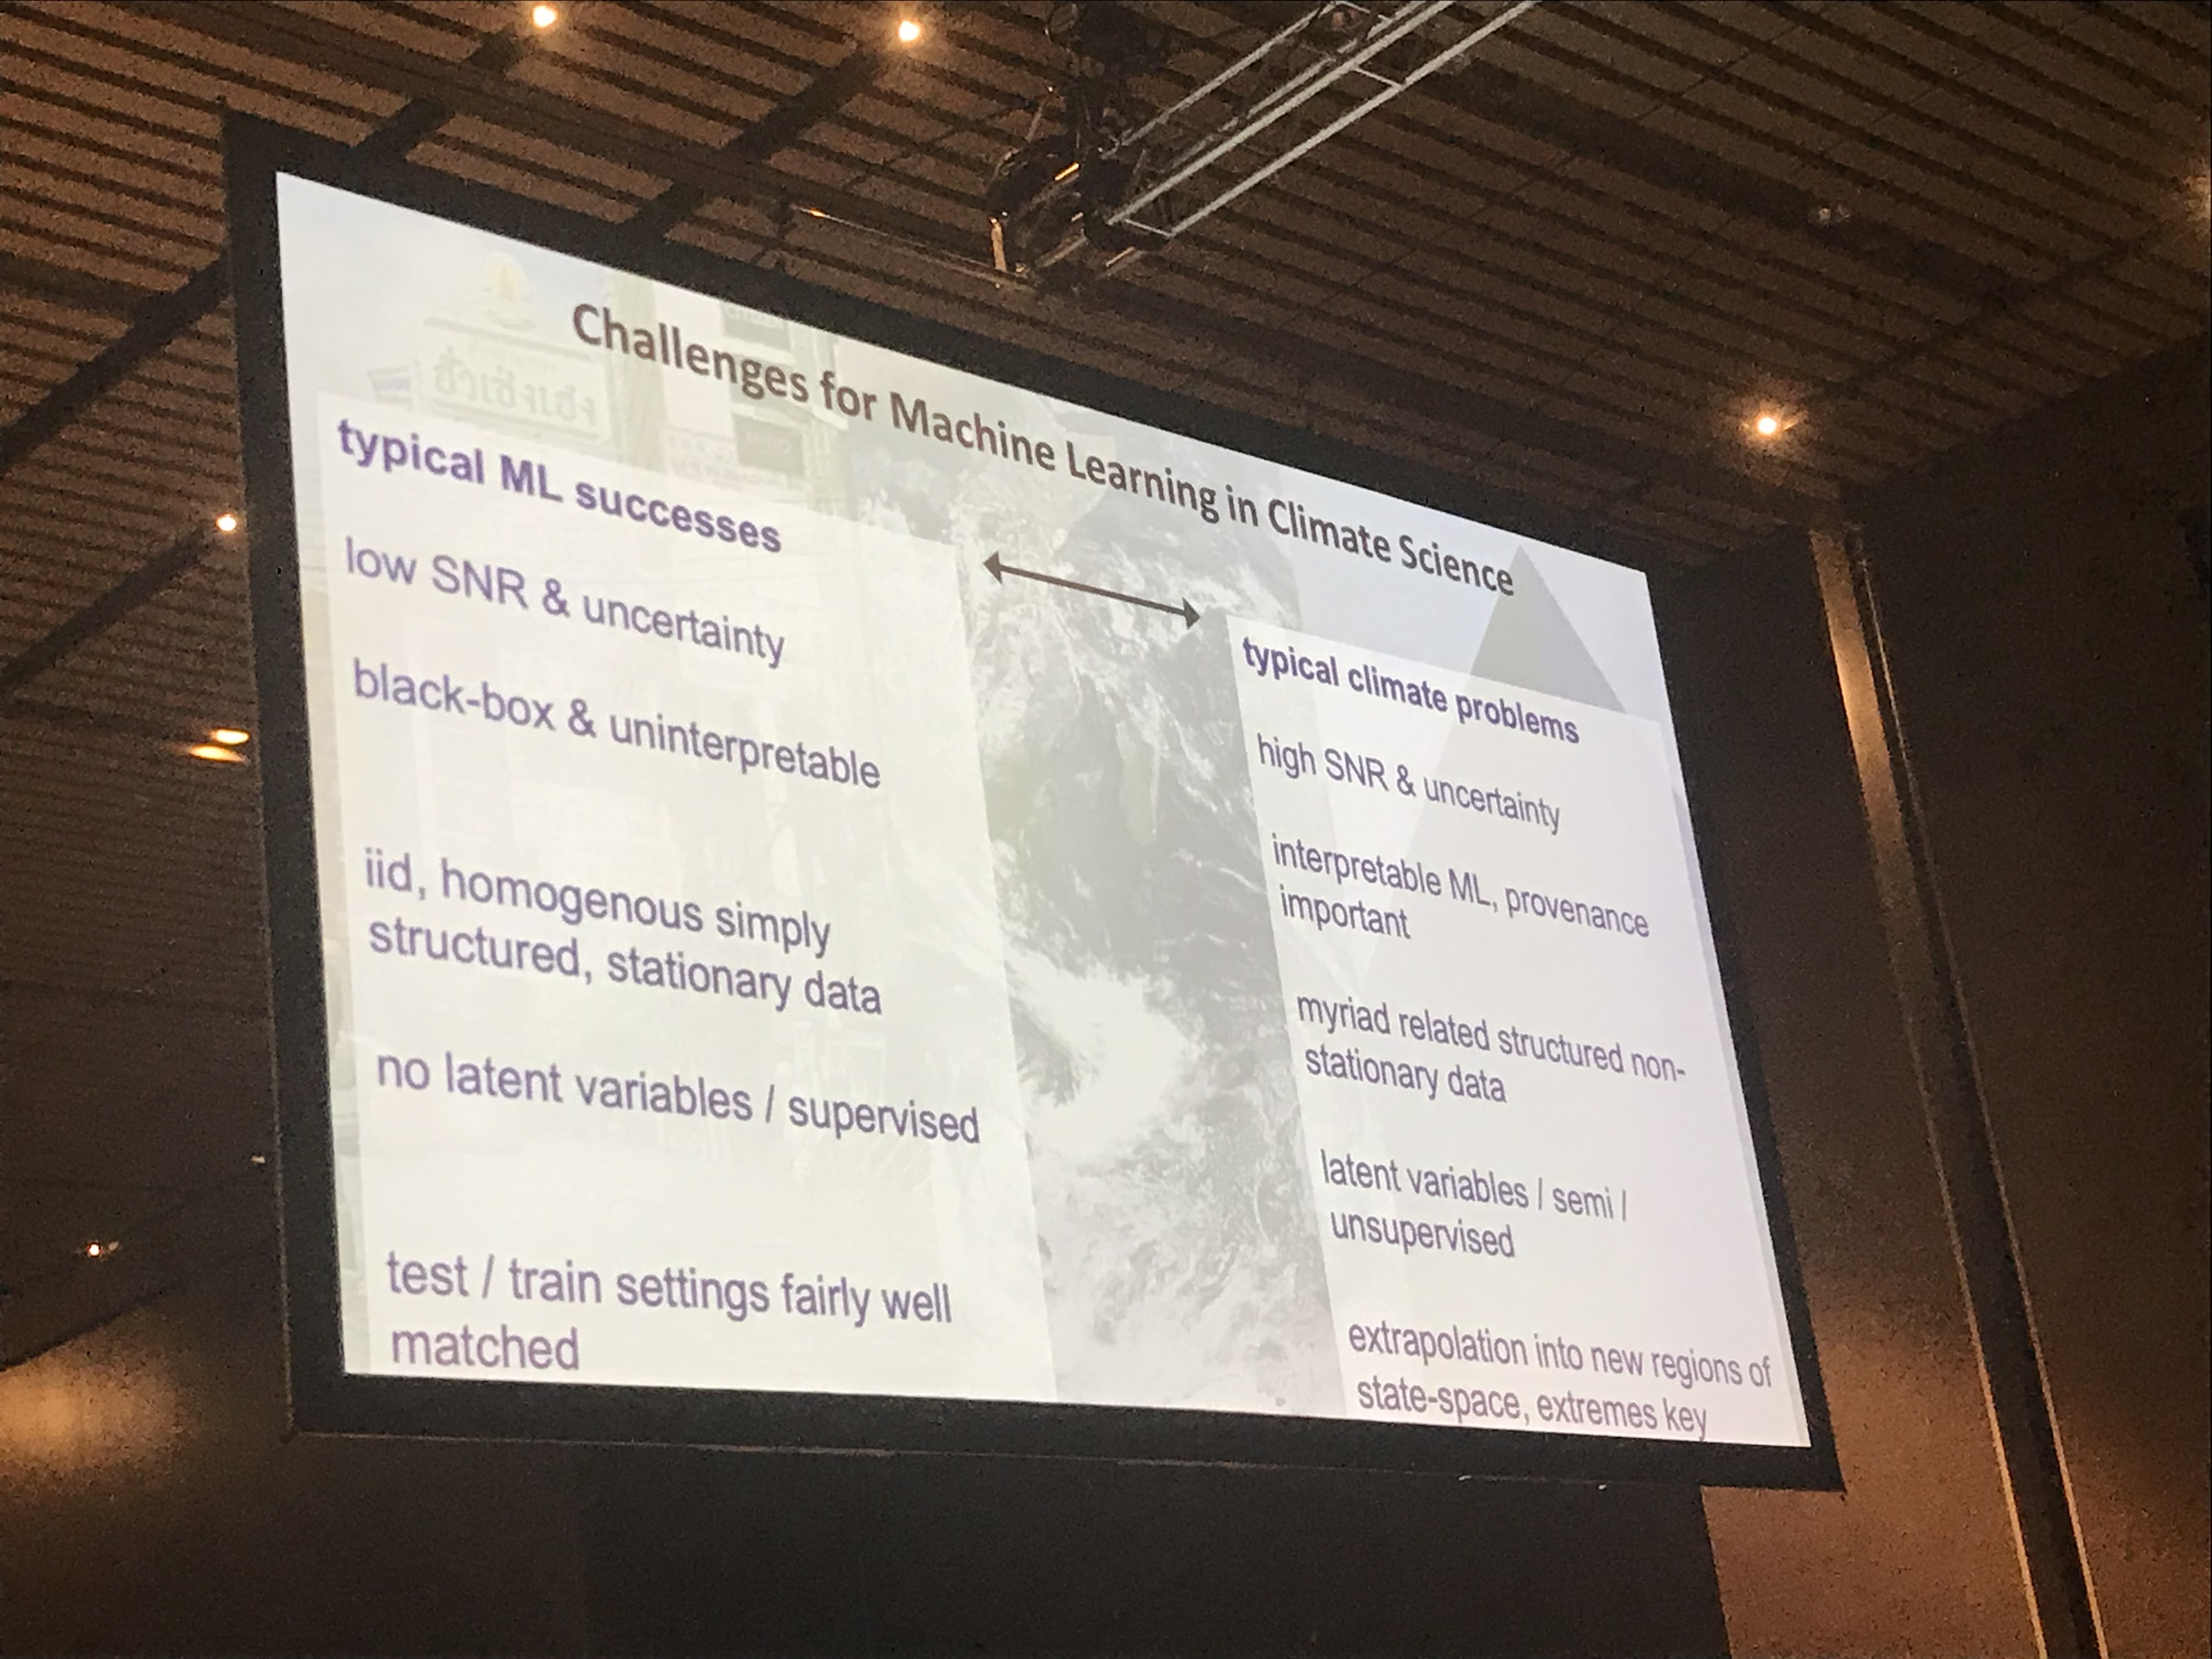
\includegraphics[width=0.4\textwidth]{images/cc_challenges.JPG}
    \caption{Challenges in bringing tools from ML to bear on problems in Climate Science.}
    \label{fig:cc_ml}
\end{figure}

Q: In spite of the challenges (see Figure~\ref{fig:cc_ml}), what can we do? \\

A: Three steps to conduct a planetary healthcheck:
\begin{enumerate}
    \item Monitoring the planet
    \item Treating the symptoms
    \item Curing the disease
\end{enumerate}

\subsubsection{Step One: Monitoring The Planet}

Q: How can we appropriately monitor the health of the planet? It's a huge challenge! Lots of important data is sparse, while less important (or low signal-noise ratio data) is abundant. \\

A: More comprehensive testing -- not just temperature, but lots of other properties, too.

\begin{figure}
    \centering
    \subfloat[Surface temperature over time]{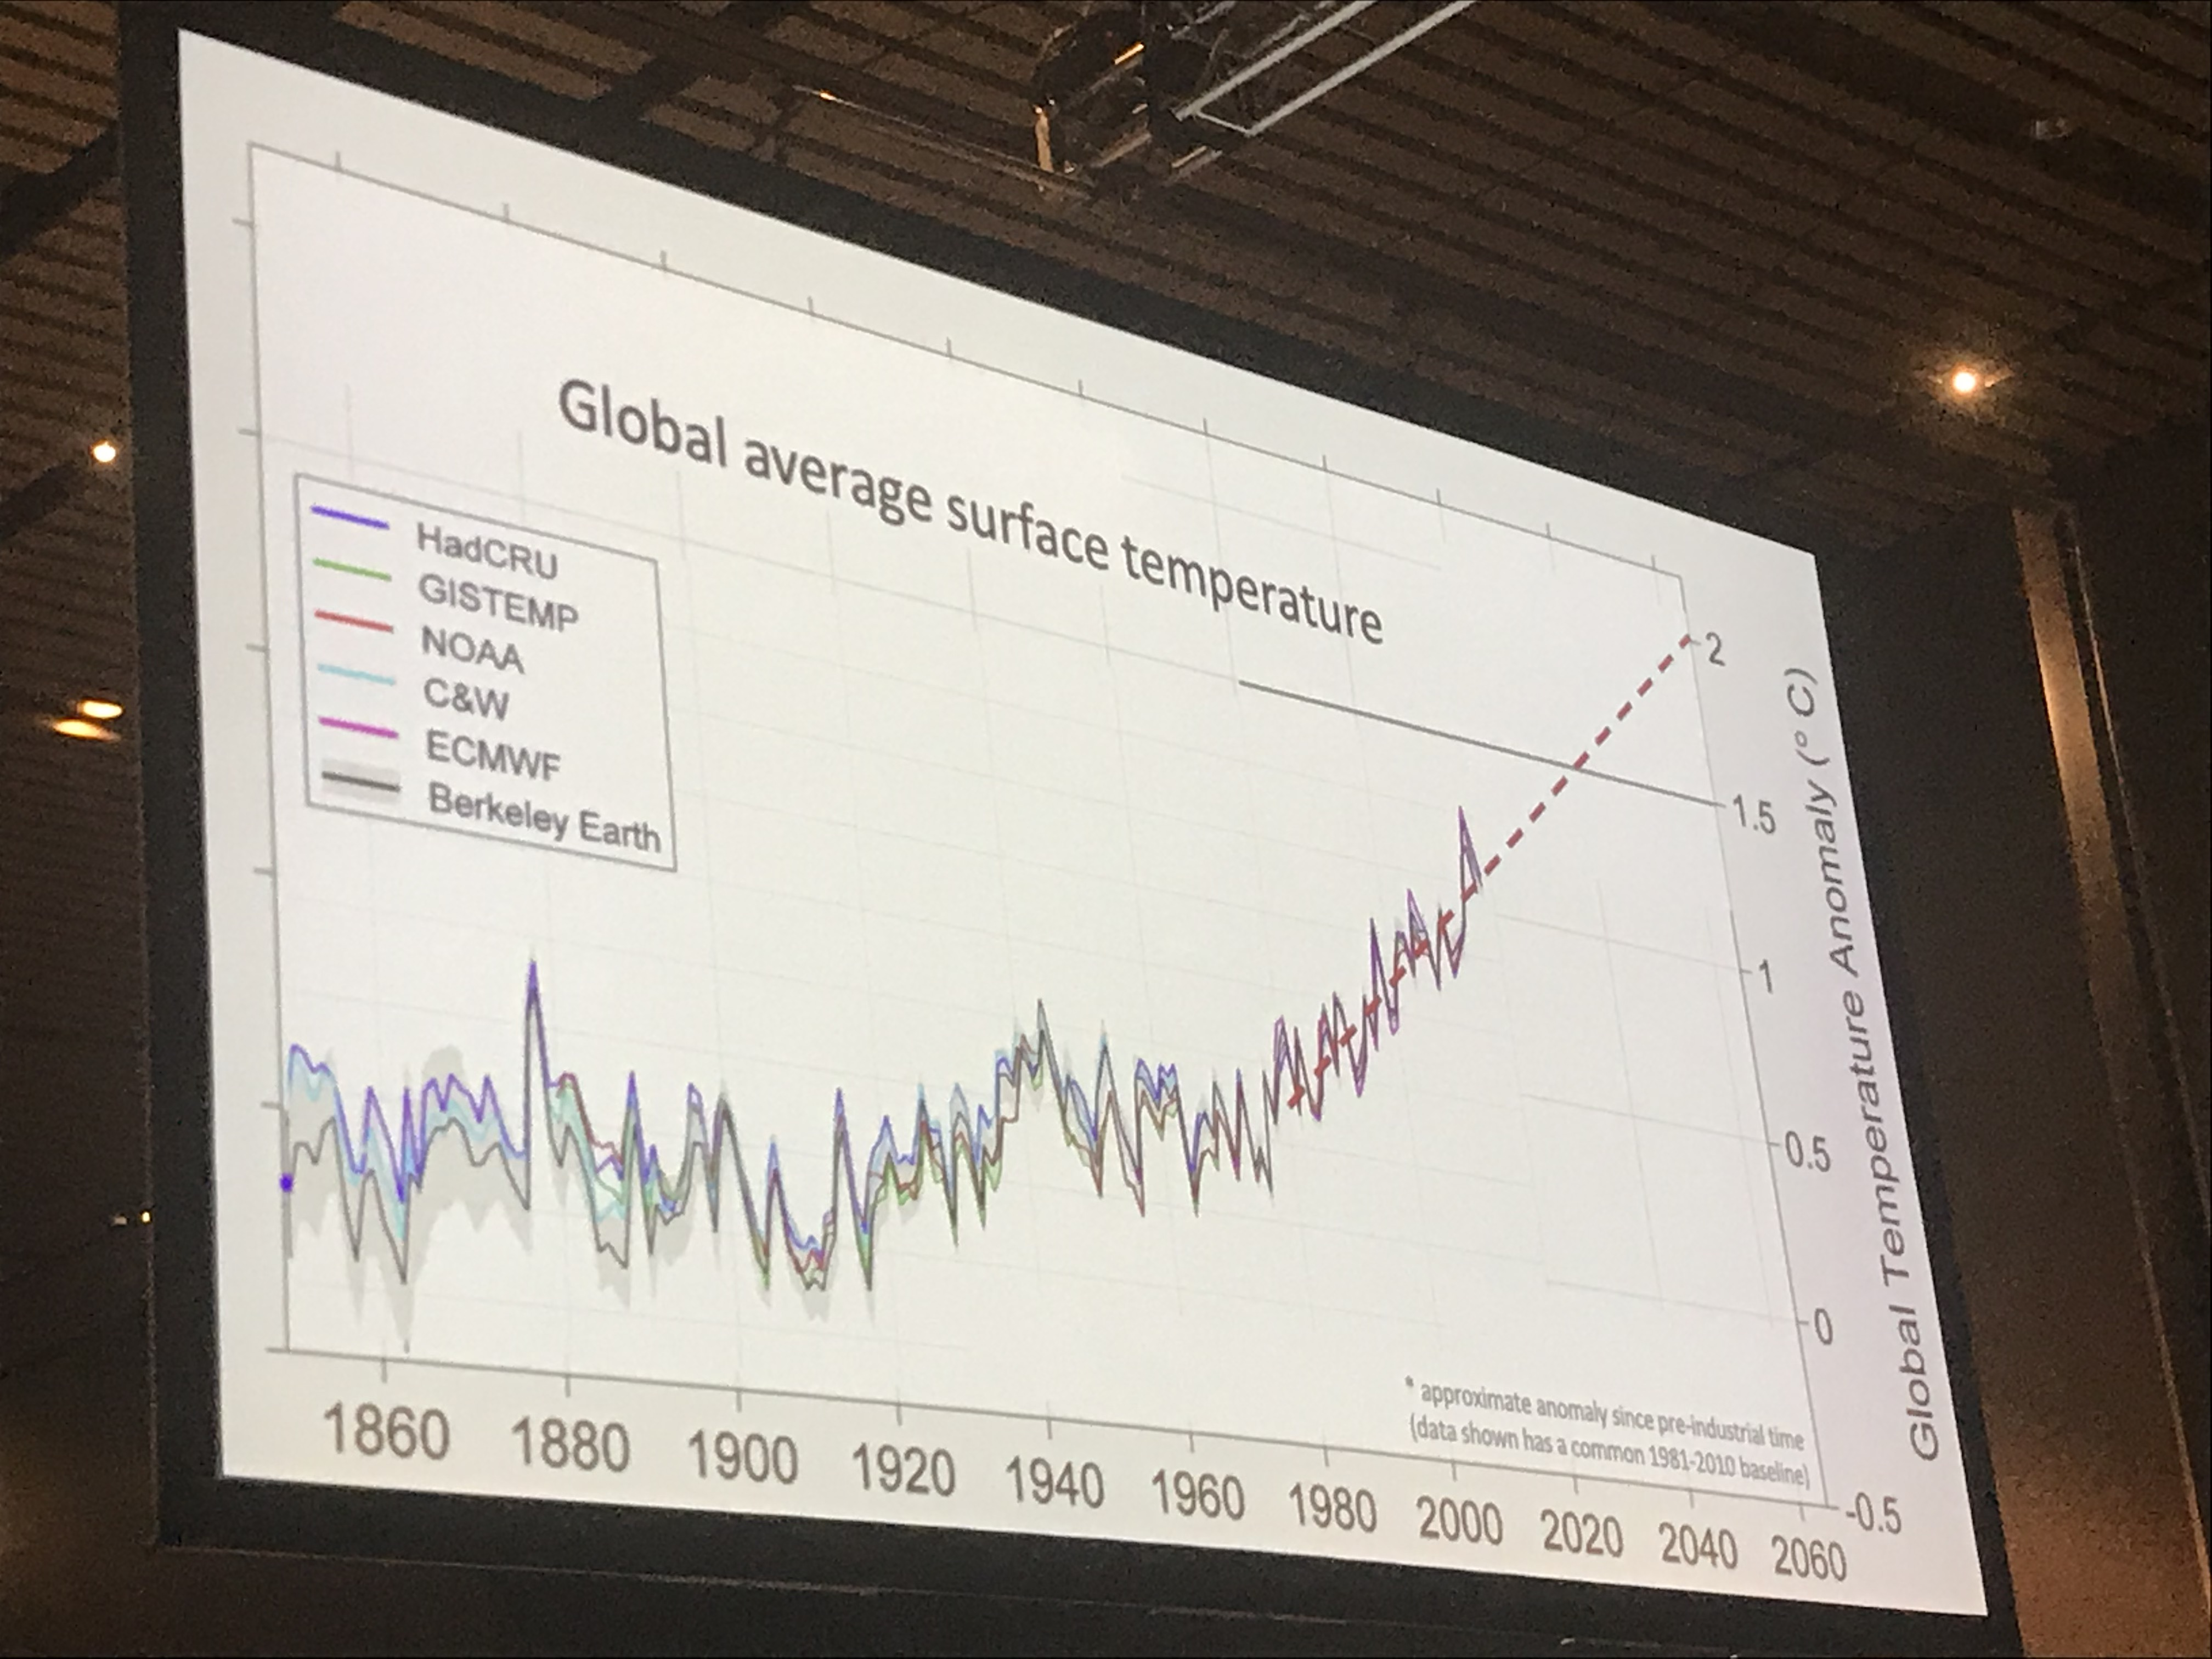
\includegraphics[width=0.4\textwidth]{images/temp.JPG}} \hspace{5mm}
    \subfloat[Other climate-relevant data over time]{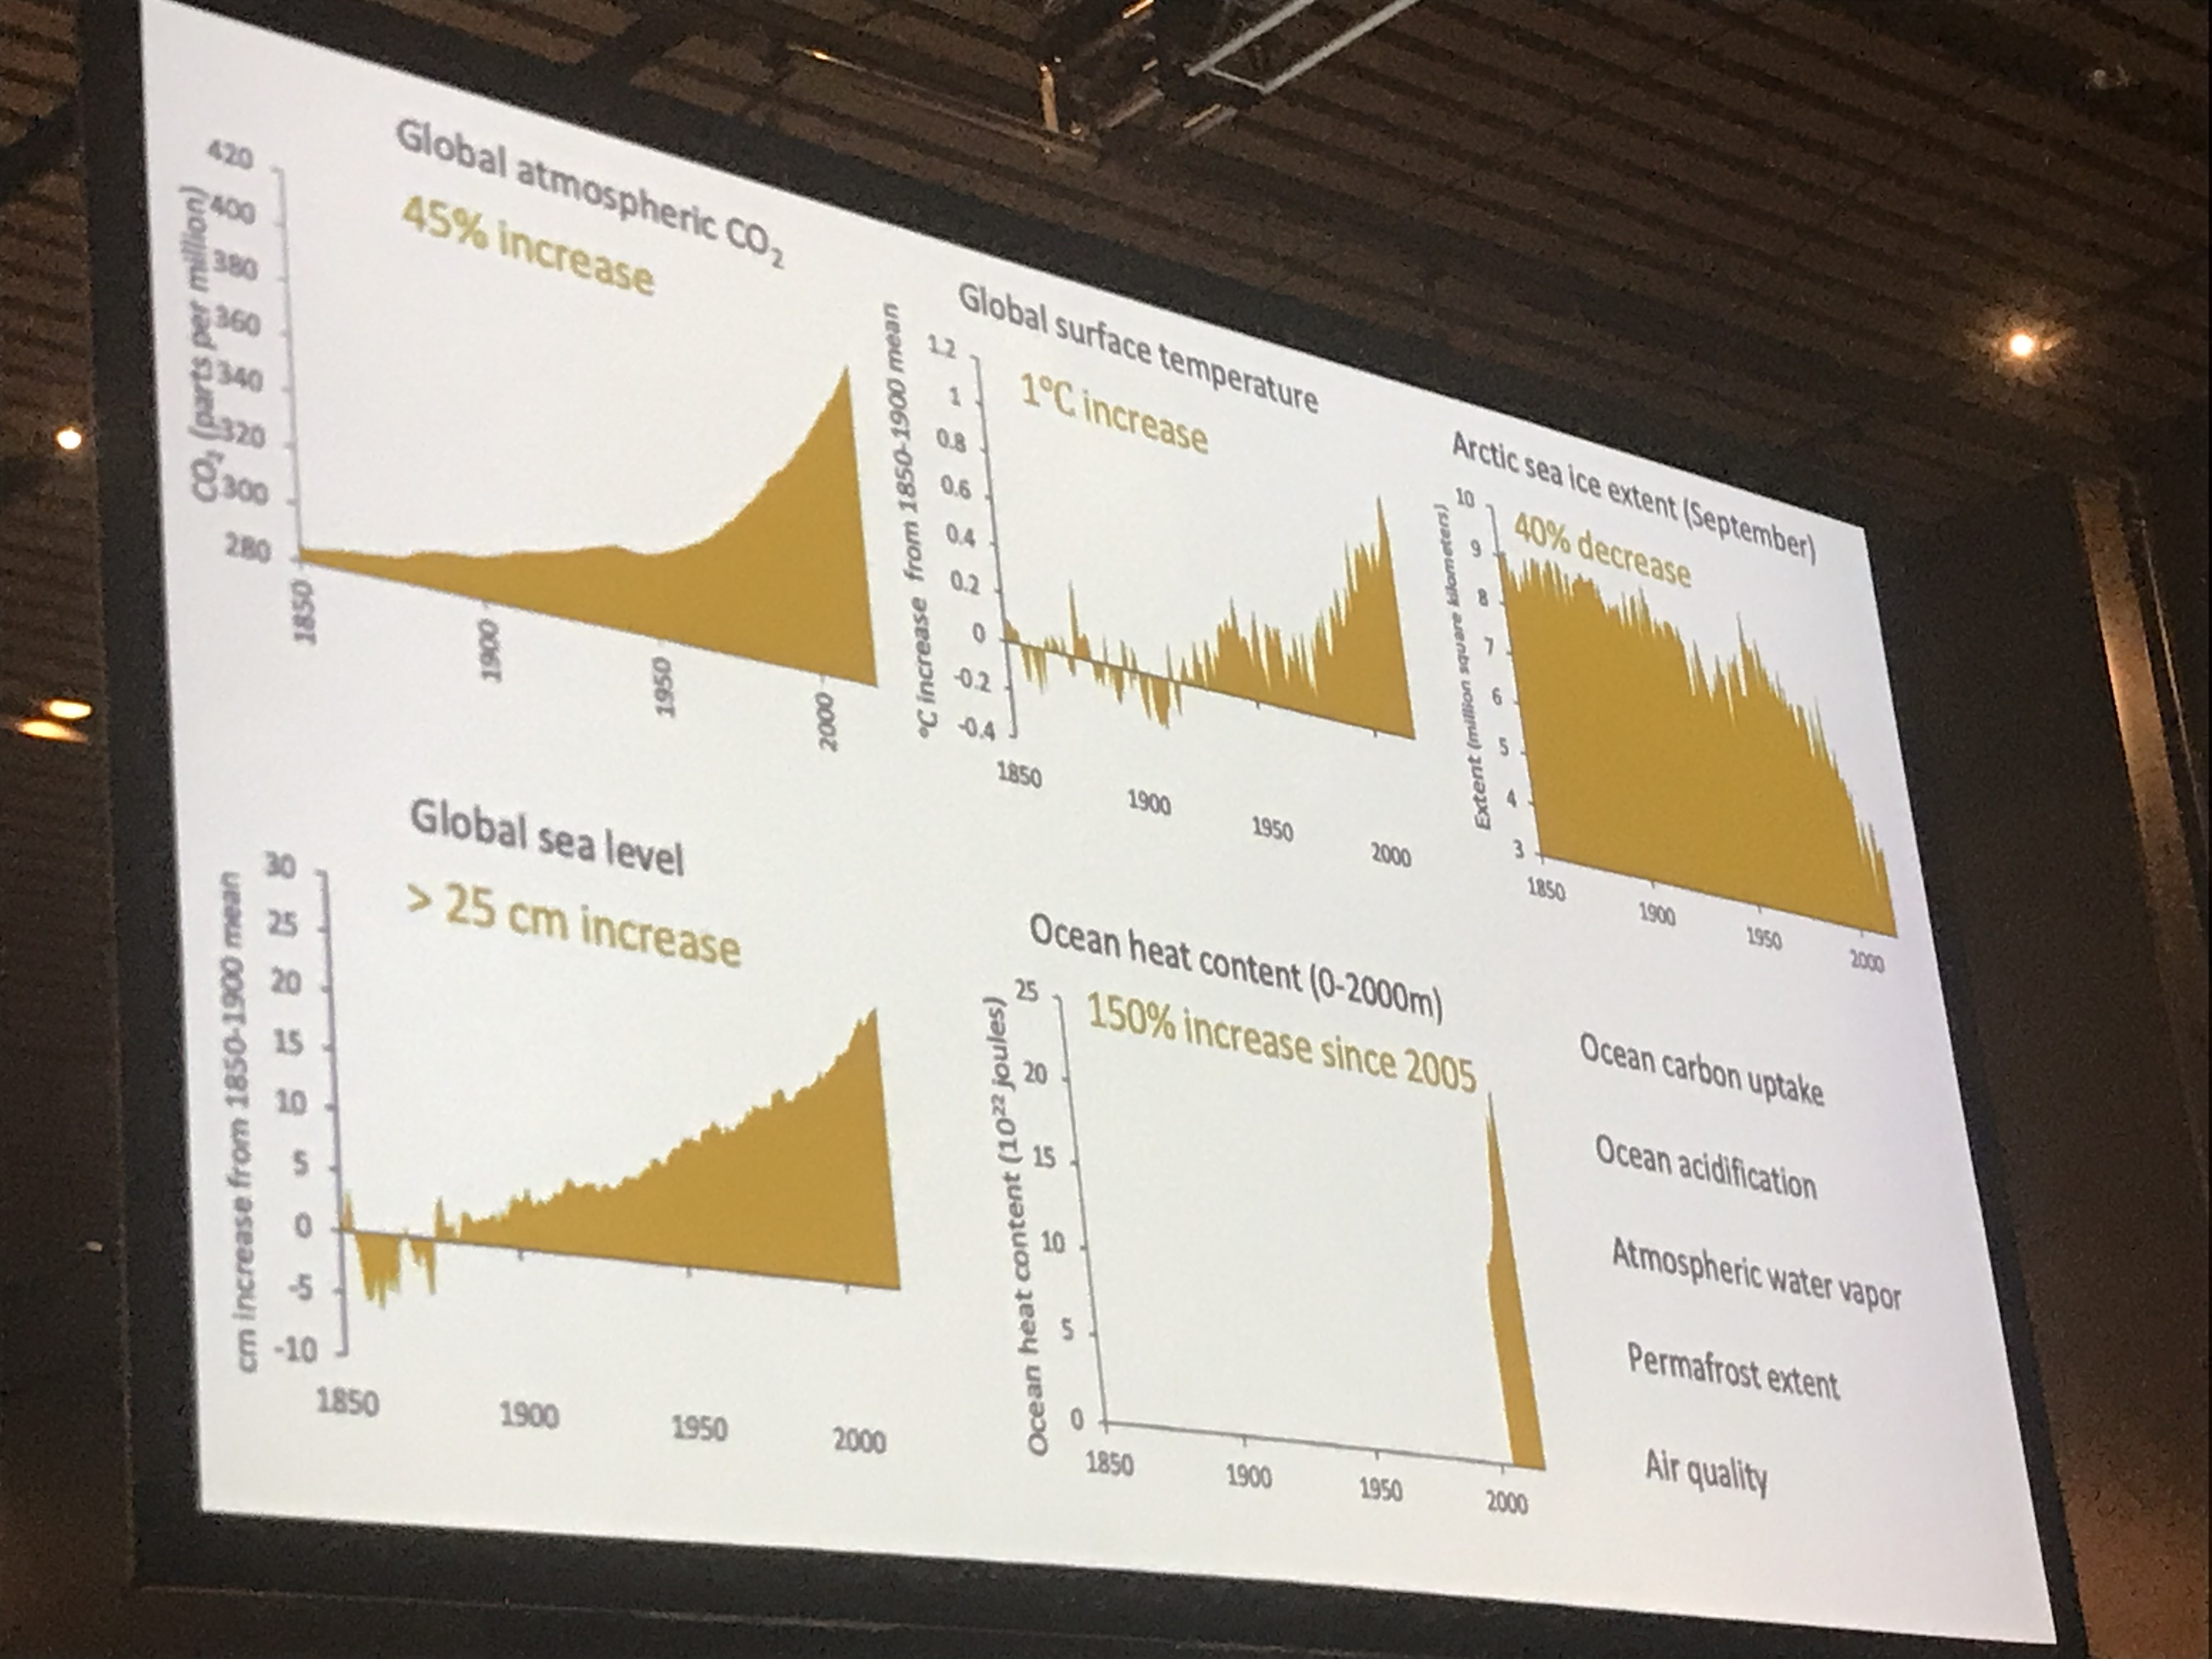
\includegraphics[width=0.4\textwidth]{images/cc_data.JPG}}
    \caption{Changes in properties of the earth's health over time.}
    \label{fig:cc_data}
\end{figure}


\subsubsection{Step Two: Treating the Symptoms}

Standard tools: co-ordinated international climate modeling project (CMIP6): \~ 40 Petabytes. Around a million lines of code, used to run simulations of surface radiation, changes in solar radiation, and so on. \\

Q: What do these models do for us? \\

A: They make predictions about critical properties in the future, like emissions due to greenhouse gases with and without different interventions, and so on. \\

$\ra$ we can actually predict global average surface temperature extremely well. \\

Q: What will future conditions be like in the world's cities and megacities? How can we predict these things? \\

A: clime models can project these changes many years into the future! \\

But: 1) have coarse resolution, 2) have systematic biases at a local level, and 3) different clime models do better/worse at representing different aspects of the climate system. \\

Example: Consider a climate model making predictions about temperatures in London. \\

$\ra$ Sometimes, the model is systematically wrong (biased). It's too high for long periods, then too low, and so on. So how can we remedy this? \\

{\bf Approach:} Apply probabilistic machine learning to build a new predictive model from actual observed weather data. That is, learn $f : \mc{X} \ra \mc{Y}$, given lots of weather data. \\

Q: Can we go further? Can we extend this model to account for correlated risks and map to data on impacts? \\

$\ra$ Really we'd like to regulate sustainable urban drainage, thermal comfort in buildings, and address questions like how vulnerable a particular country/region is to clime disruption? \\

Similar approach---consider a task where: \\
\hspace{8mm}{\bf input:} time, space, climate model outputs, meteorological data
\hspace{8mm}{\bf output}: future risk of specific impact occurring, with the {\bf task:} of synthesizing and interpolating different datasets, learn mappings between different variables, may need to find novel sources of data.\\

\subsubsection{Step Three: Cure the Disease}

{\bf Key Takeaway:} many opportunities for improve future projections of climate change to inform policymaking. Here are a few:

\begin{enumerate}
    \item Blend data-driven and physics based approaches
    
    $\ra$ Can combine physics models of ice melt and machine learning models (with our large dataset) to make more accurate predictions of ice melt.
    
    \item Develop data-based simulators of key processes
    
    $\ra$ Given massive datasets of key processes, such as cloud formations, we can help to build more accurate models. Current climate models don't scale well, so we need to find new ways to model climate change.
    
    \item Use ML to better understand the {\it physical processes} involved in key shifts, as in glacier shifts (see Figure~\ref{fig:glacier}.
    
\end{enumerate}

\begin{figure}
    \centering
    \subfloat[]{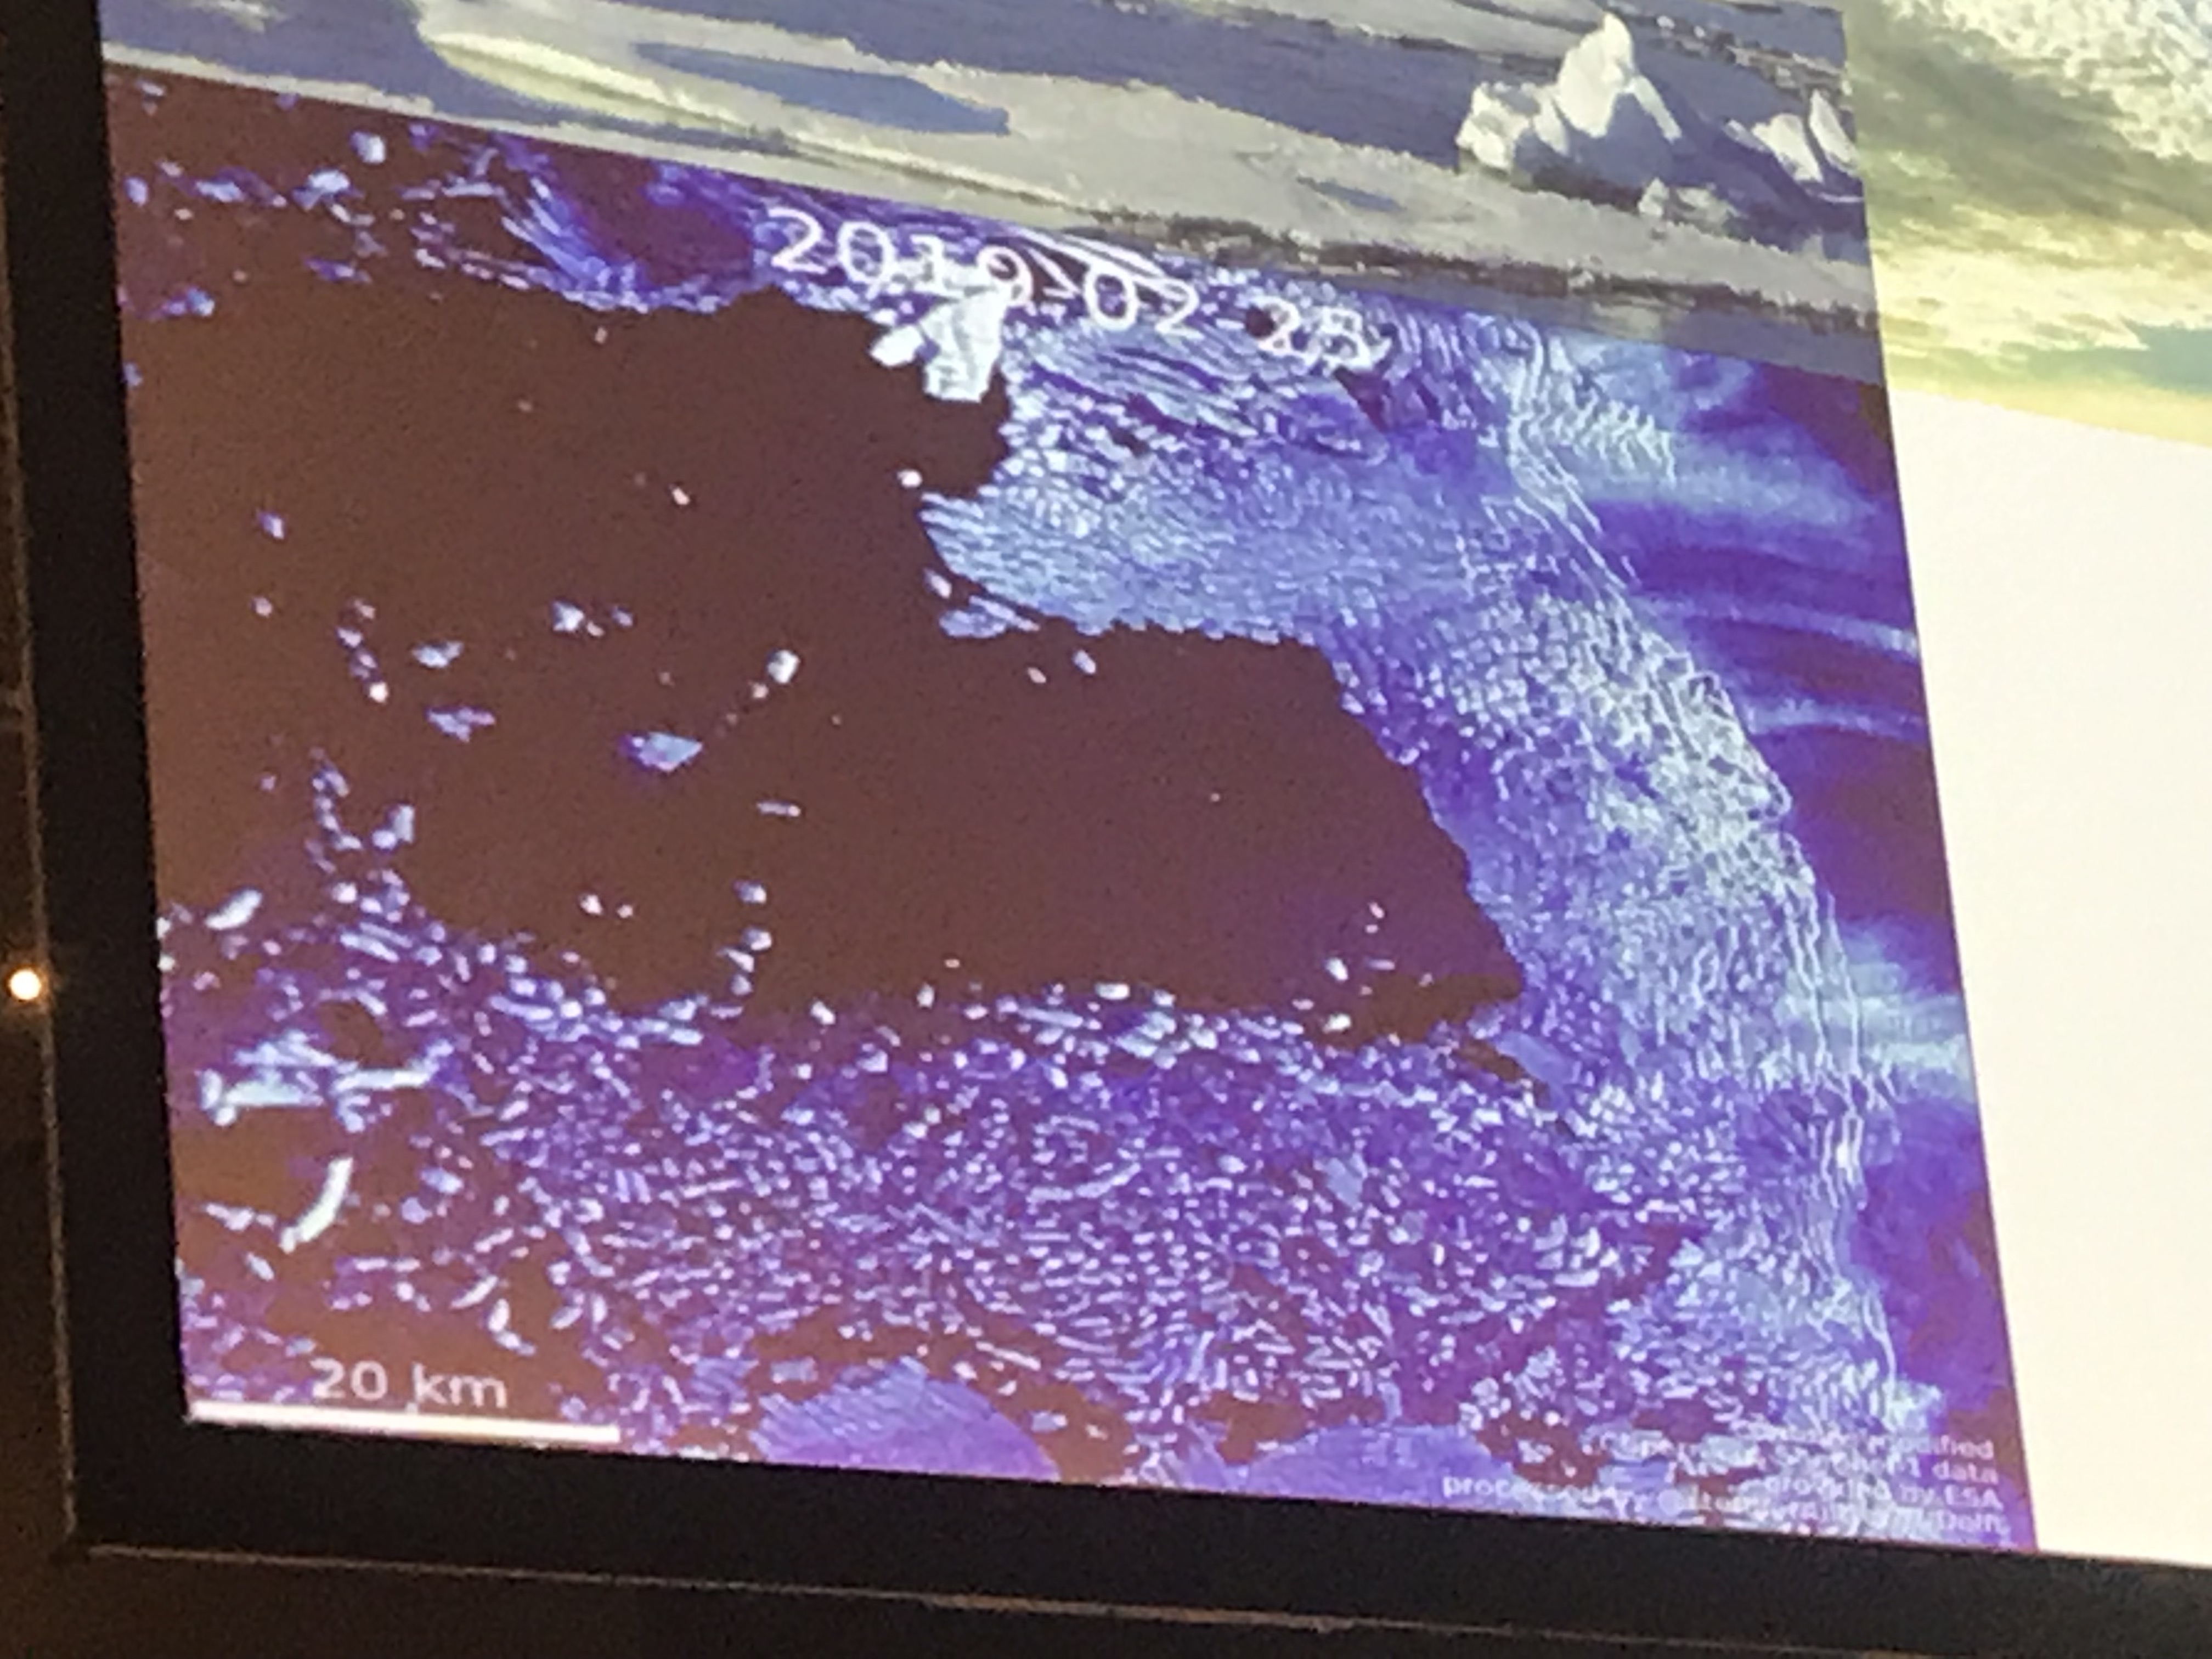
\includegraphics[width=0.29\textwidth]{images/glacier_1.JPG}} \hspace{3mm}
    \subfloat[]{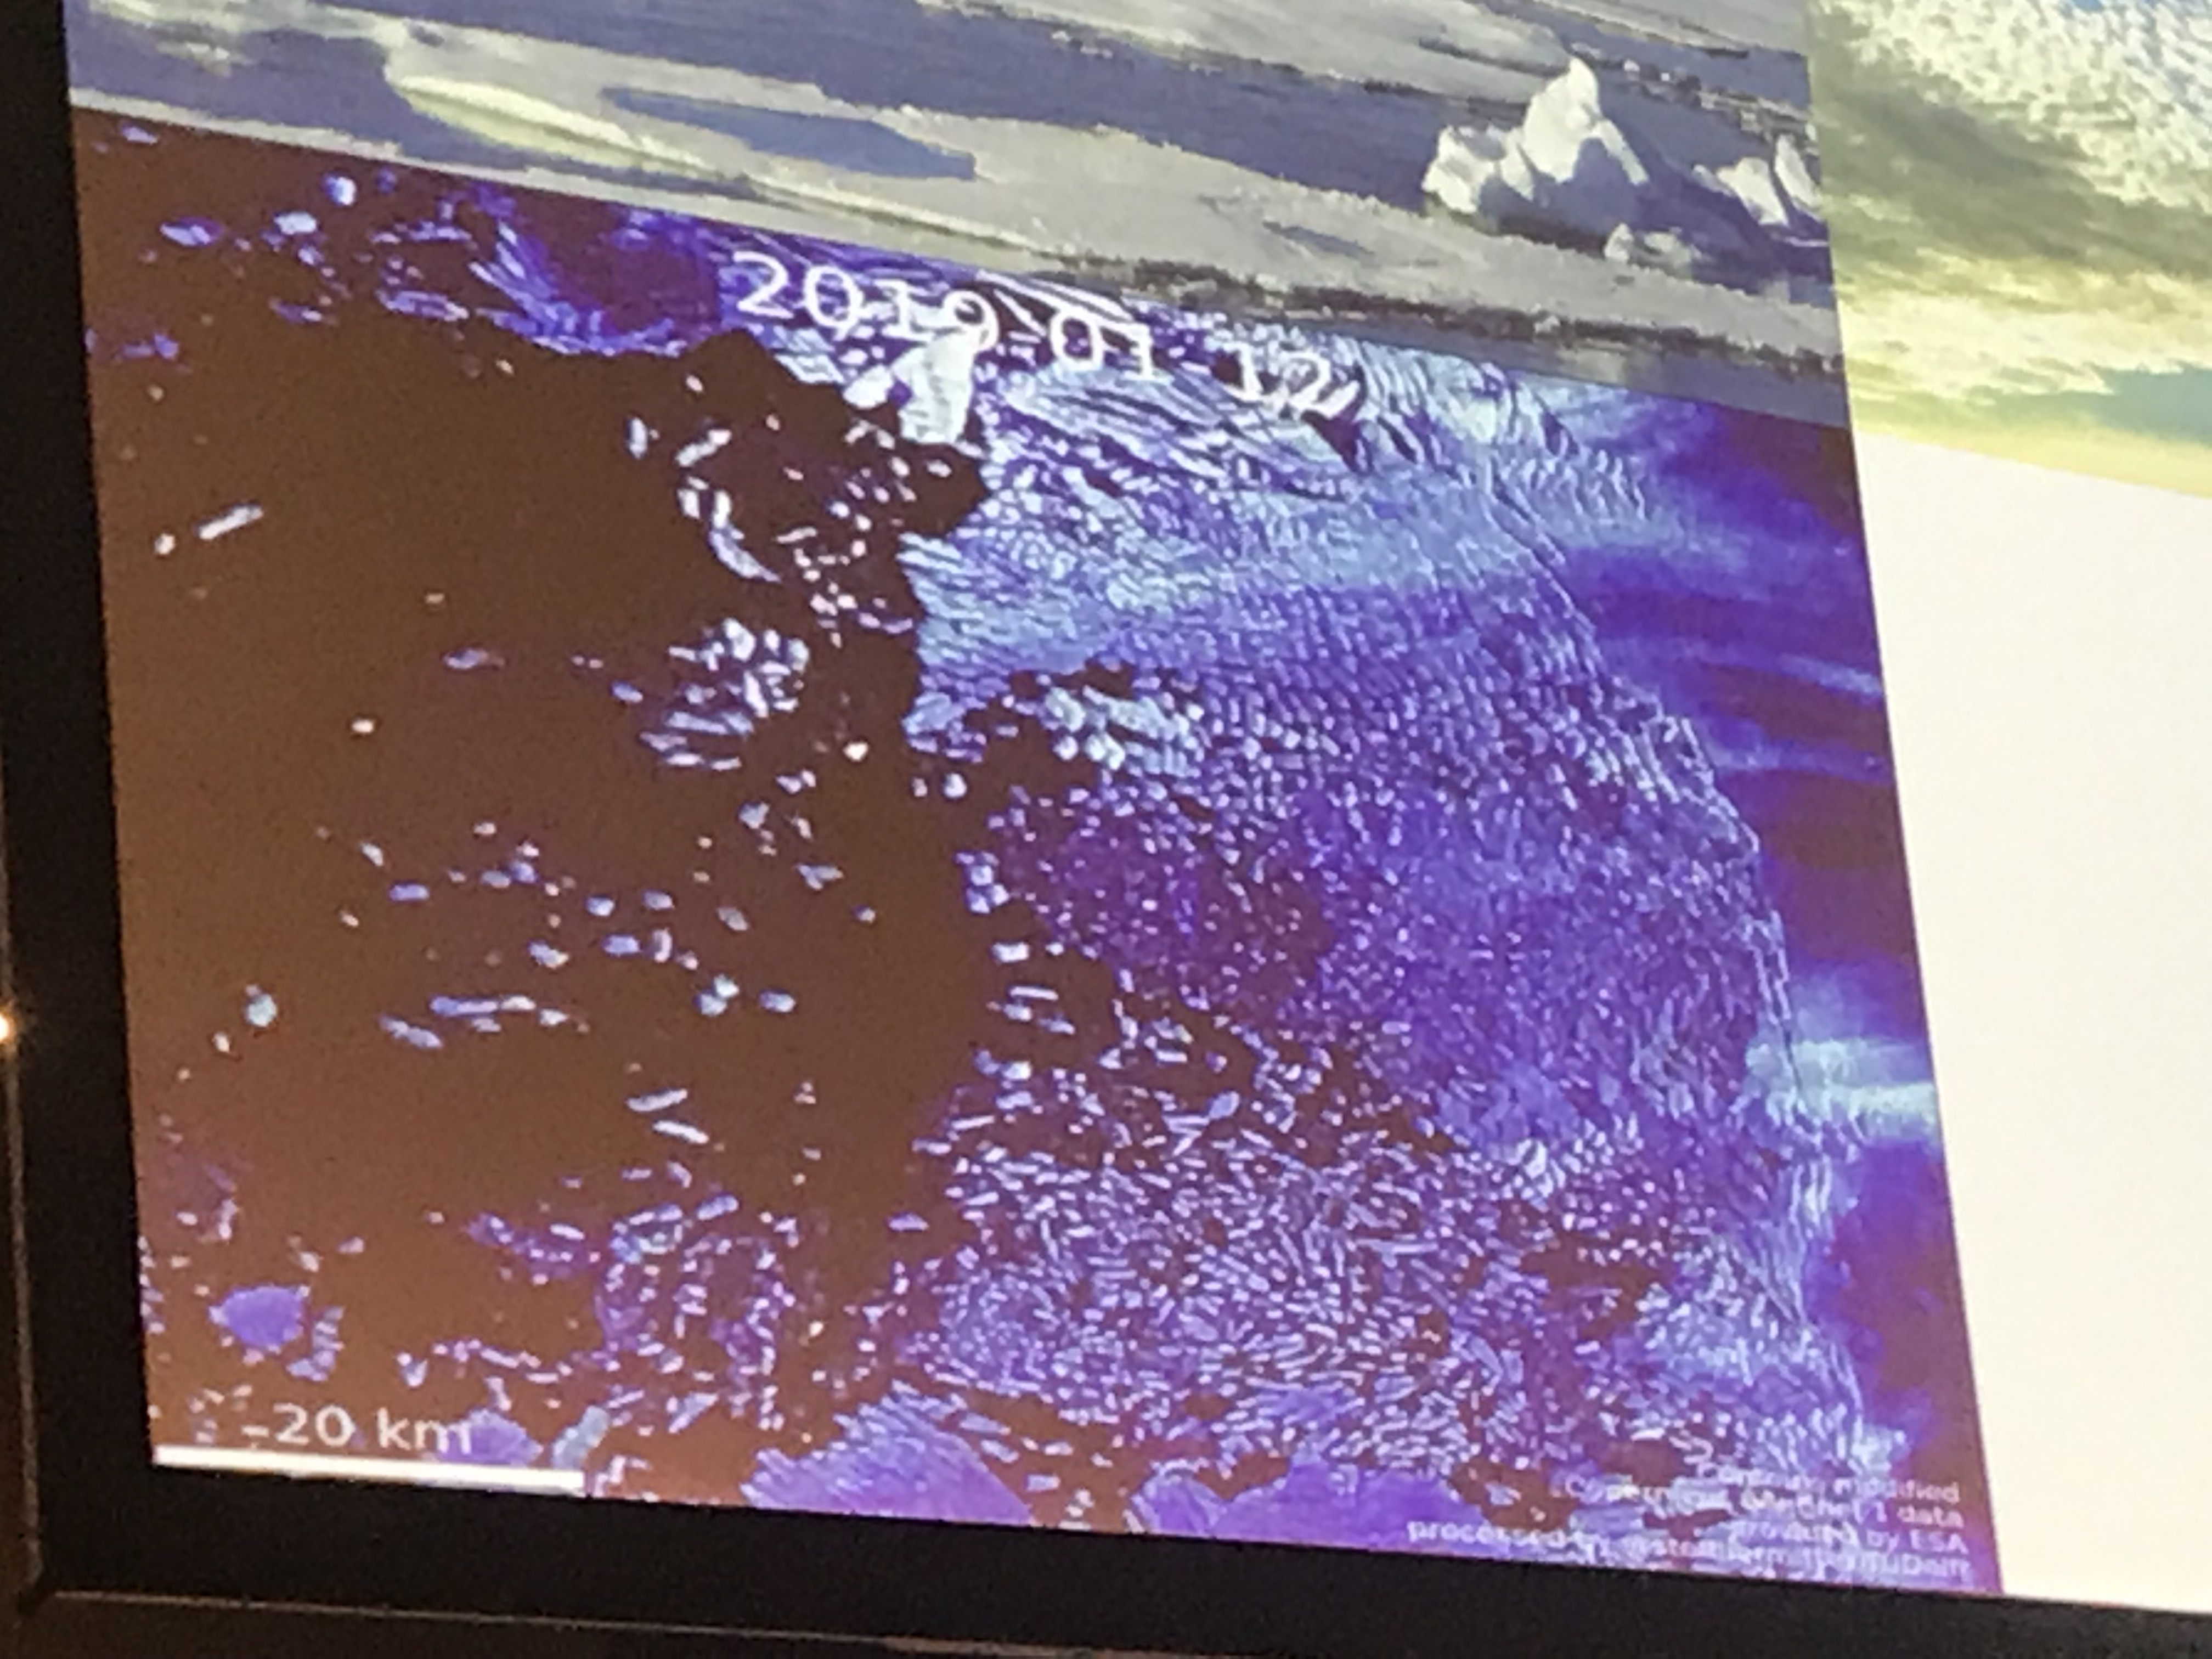
\includegraphics[width=0.29\textwidth]{images/glacier_2.JPG}} \hspace{3mm}
    \subfloat[]{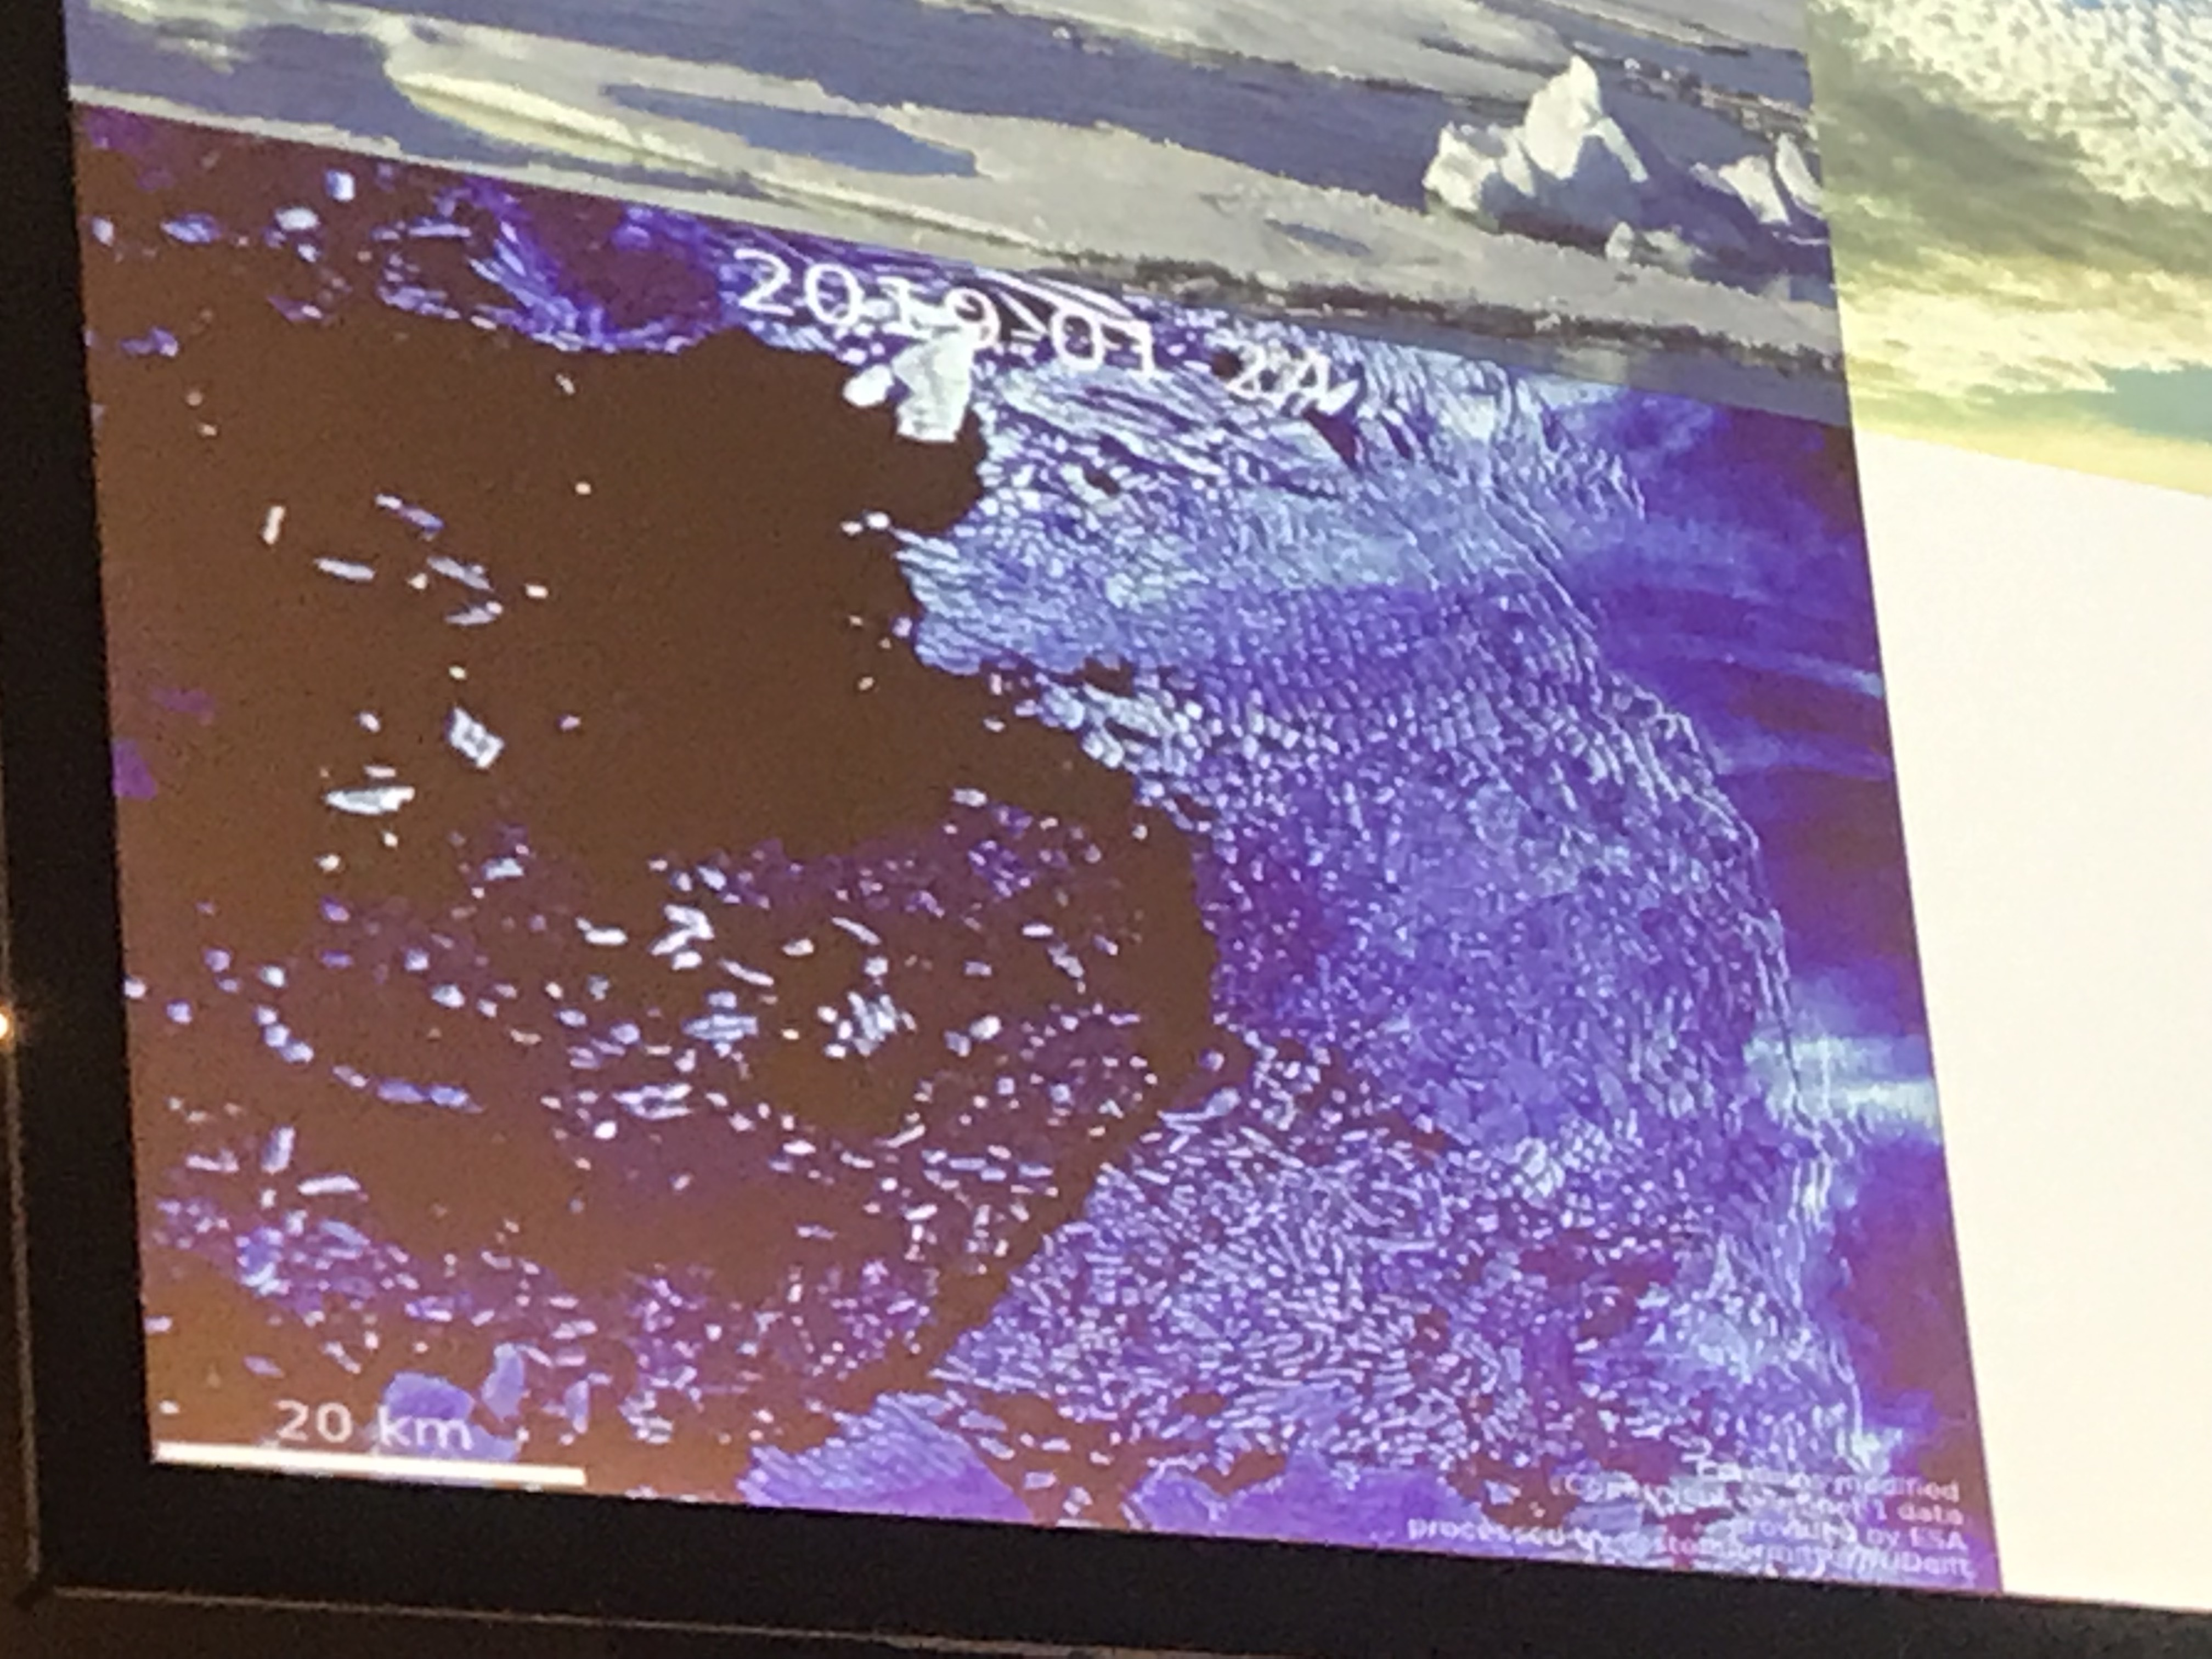
\includegraphics[width=0.29\textwidth]{images/glacier_3.JPG}} \hspace{3mm}
    \caption{Change in glacial structure over time.}
    \label{fig:glacier}
\end{figure}

Summary:
\begin{enumerate}
    \item Climate change is perhaps the defining issue of our time
    \item To assess risks posed to society and the natural world, we need more information and tools.
    \item Vast datasets cover every aspect of the planet's health but we lack some of the {\it tools} tp process them to generate that information.
    
    \item {\bf Takeaway Question:} Can we establish benchmark tasks that drive climate research forward much like ImageNet has done for vision?
\end{enumerate}

\dnote{Stepping out for meetings the rest of the day, back at it tomorrow!}